\section{Modi naturali per i sistemi dinamici}
I modi naturali sono tutte le funzioni che possono comparire nella risposta in
evoluzione libera, ovvero tutte le funzioni del tempo che possono essere
identificate all'interno della matrice esponenziale
$$
x_l(t) = e^{At}x_0\ x_0 \in \mathbb{X}^n
$$

Si consideri un sistema con $n=3$ con i seguenti autovalori e autovettori della
matrice della dinamica $A$:
$$\begin{array}{ccc}
\lambda & \alpha+j\omega & \alpha-j\omega\\
\downarrow &\downarrow &\downarrow \\
u & u_a +j u_b & u_a -j u_b
\end{array}$$

Si costruisce la matrice modale reale $U_r$ e la sua inversa $U_r^{-1}$
$$\begin{aligned}
U_r &= [u \ u_a \ u_b] \\
U_r^{-1} &= \begin{bmatrix}
             v^T\\v_a^T\\v_b^T
            \end{bmatrix}
\end{aligned}$$

Si introduce il cambio di variabili con una nuova variabile di stato $z$
$$
z = U_r^{-1} x\rightarrow \Lambda_r = U_r^{-1}AU_r = \left(
\begin{array}{c:cc}
 \lambda & 0 & 0 \\ \hdashline
 0 & \alpha & \omega \\
 0 & -\omega & \alpha
\end{array}
\right)
$$

Calcolando la matrice esponenziale si ottiene
$$
e^{At} = e^{\left(U_r\Lambda_r U_r^{-1} \right)t} = U_r e^{\Lambda_r t}U_r^{-1}
= \begin{pmatrix}
   u & u_a & u_b
  \end{pmatrix}\left(
\begin{array}{c:c}
 e^{\lambda t}& 0 \quad 0 \\ \hdashline
\begin{aligned}
0 \\ 0
\end{aligned} &\begin{aligned} \\ e^{\begin{pmatrix}
\alpha& \omega\\
-\omega & \alpha
\end{pmatrix}t}\end{aligned}
\end{array}\right)
\begin{pmatrix}
v^T \\ v_a^T \\ v_b^T
\end{pmatrix}
$$
Sviluppando l'esponenziale interno
$$
e^{\begin{pmatrix}
\alpha& \omega\\
-\omega & \alpha
\end{pmatrix}t} =
e^{\alpha t} \begin{pmatrix}
              \cos \omega t & \sin \omega t \\
              -\sin \omega t & \cos \omega t
             \end{pmatrix}
$$
La matrice esponenziale completa dunque:
$$
e^{At} = \begin{pmatrix}
   u & u_a & u_b
  \end{pmatrix}
\begin{pmatrix}
e^{\lambda t} & 0 & 0 \\
0 & e^{\alpha t}\cos\omega t & e^{\alpha t}\sin\omega t \\
0 & -e^{\alpha t}\sin\omega t & e^{\alpha t}\cos\omega t
\end{pmatrix}
\begin{pmatrix}
v^T \\ v_a^T \\ v_b^T
\end{pmatrix}
$$
Ricordando la definizione di modo naturale si vede che le funzioni del tempo
sono tutte contenute nella matrice esponenziale degli autovalori
$e^{\Lambda_r t}$

Si sviluppano i prodotti
$$
e^{At} = e^{\lambda t}uv^T + e^{\alpha t}u_a \left(\cos(\omega t) v_a^T +
\sin(\omega t)v_b^T \right)+
e^{\alpha t}u_b \left(-\sin(\omega t) v_a^T +
\cos(\omega t)v_b^T \right)
$$

Si considera ora l'evoluzione libera
$$\begin{aligned}
x_l(t) &= e^{At}x_0 = e^{\lambda t} uv^Tx_0 + e^{\alpha t}\left[
u_a \left(\cos(\omega t) v_a^Tx_0 +
\sin(\omega t)v_b^Tx_0 \right) +\right. \\
 &\left.+ e^{\alpha t}u_b \left(-\sin(\omega t) v_a^Tx_0 +
\cos(\omega t)v_b^Tx_0 \right)
\right]
\end{aligned}$$
si osserva che i vettori $v^T$ sono righe mentre $x_0$ sono vettori colonna, di
conseguenza il loro prodotto è uno scalare $c$, si fanno le seguenti posizioni
$$
\begin{bmatrix}
v^T \\ v_a^T \\ v_b^T
\end{bmatrix}
x_0 =
\begin{pmatrix}
 c \\ c_a \\  c_b
\end{pmatrix}
$$
Si riscrive l'equazione dell'evoluzione libera
$$\begin{aligned}
x_l(t) &= ce^{\lambda t}u +e^{\alpha t} u_a\left(\cos(\omega t)c_a +
\sin(\omega t) c_b\right) + \\
& + e^{\alpha t} u_b\left(-\sin(\omega t)c_a +
\cos(\omega t) c_b\right)
\end{aligned}$$
Se si analizza lo stato nell'istante di tempo nullo
$$
x_l(0) = cu + c_au_a +c_bu_b =x_0 \Rightarrow z_l(0) = \begin{pmatrix}
 c \\ c_a \\  c_b
\end{pmatrix} = z_0 = U_R^{-1} x_0
$$
Si osserva che le costanti $c$ sono proprio le componenti dello stato iniziale
rispetto alla nuova base $u$.

Si considerino le seguenti posizioni per definire l'angolo $\varphi$
$$
m=\sqrt{c_a^2 + c_b ^2} \qquad \sin\varphi = \frac{c_a}{m} \qquad \cos\varphi =
\frac{c_b}{m}
$$
si riscrive la $x_l(t)$ in forma ancora più compatta, sfruttando le formule di
prostaferesi
$$
x_l(t) = ce^{\lambda t} u + me^{\alpha t}\left(\sin(\omega t +\varphi)u_a +
\cos(\omega t + \varphi)u_b\right)
$$
Le funzioni dipendenti dal tempo, generate da matrici diagonalizzabili, possono
essere al più esponenziali scalari per ogni autovalore reale, chiamati moti
\textbf{aperiodici}; oppure funzioni sinusoidali moltiplicate per esponenziali
per ogni autovalore complesso e coniugato, verranno detti modi
\textbf{pseudo-periodici}.

Si vuole capire come sarà l'andamento qualitativo dell'evoluzione libera dello
stato al variare degli autovalori.

\newpage
\subsection{Modi aperiodici}
Sono generati da autovalori reali
$$
\lambda \text{ reali} \rightarrow e^{\lambda t} u
$$
Si possono avere tre casi
\begin{figure}[h]
\centering
 \begin{subfigure}[b]{0.32\textwidth}
  \centering
  \begin{tikzpicture}
   \begin{axis}[
     axis lines=left,
     width=\textwidth,
     xtick={0,1,3.5},
     xticklabels={0,$\tau$,t},
     ytick={1,1.5},
     ymax=1.5,
     yticklabels={1,$x_l(t)$},
     ]
    \addplot[color=black,domain=0:3.5]{exp(-x)};
    \addplot[color=black,domain=0:1]{1-x};
   \end{axis}
  \end{tikzpicture}
  \caption{$\lambda<0$}
 \end{subfigure}
\hfill
 \begin{subfigure}[b]{0.32\textwidth}
  \centering
  \begin{tikzpicture}
   \begin{axis}[
     axis lines=left,
     width=\textwidth,
     xtick={0,3.5},
     xticklabels={0,t},
     ytick={1,1.5},
     ymax=1.5,
     ymin = 0,
     yticklabels={1,$x_l(t)$},
     ]
    \addplot[color=black,domain=0:3.5]{1};
   \end{axis}
  \end{tikzpicture}
  \caption{$\lambda=0$}
 \end{subfigure}
\hfill
 \begin{subfigure}[b]{0.32\textwidth}
  \centering
  \begin{tikzpicture}
   \begin{axis}[
     axis lines=left,
     width=\textwidth,
     xtick={0,3.5},
     xticklabels={0,t},
     ytick={1,34},
     ymax=34,
     ymin = 0,
     yticklabels={1,$x_l(t)$},
     ]
    \addplot[color=black,domain=0:3.5]{exp(x)};
   \end{axis}
  \end{tikzpicture}
  \caption{$\lambda>0$}
 \end{subfigure}
\end{figure}

Nello spazio di stato $X^n$ si individua una direzione data dal vettore $u$,
all'istante $t=0 \rightarrow e^{\lambda t}u = u$, non c'è alcun contributo
dato dal modo.

Al variare di $t$ il vettore $u$ può
\begin{itemize}
\item $\lambda<0$ il vettore diminuisce di ampiezza.
\item $\lambda=0$ il vettore resta costante.
\item $\lambda>0$ il
vettore aumenta di ampiezza indefinitamente.
\end{itemize}

Se $\lambda<0$ si introduce una \textbf{costante di tempo} $\tau =
-\frac{1}{\lambda}$
e la funzione esponenziale si può esprimere come
$e^{-\frac{t}{\tau}}$, dunque si può affermare che con una certa percentuale di
errore la funzione è ingegneristicamente approssimabile a zero.
Al variare di $\tau$ si ha un tempo di ``riduzione'' del fenomeno maggiore o
minore, per un tempo pari a tre $\tau$ il vettore si riduce di almeno il 95\%
$$\begin{aligned}
t=3\tau&\Rightarrow e^{-\frac{t}{\tau}}
< 0.05\ (5\%)\\
t=4\tau&\Rightarrow e^{-\frac{t}{\tau}}
< 0.02\ (2\%)\\
t=5\tau&\Rightarrow e^{-\frac{t}{\tau}}
< 0.01\ (1\%)
\end{aligned}$$

\newpage
\subsection{Modo Pseudo-Periodico}
Si considera una coppia di autovalori complessi e coniugati
$$
\alpha \pm j\omega \rightarrow e^{\alpha t}\left(\sin(\omega t + \varphi)u_a +
\cos(\omega t + \varphi)u_b\right)
$$

Si hanno anche in questo caso tre modi al variare di $\alpha$

\begin{figure}[h]
\centering
 \begin{subfigure}[b]{0.32\textwidth}
  \centering
  \begin{tikzpicture}
   \begin{axis}[
     axis lines=left,
     axis x line=middle,
     width=\textwidth,
     xtick={0,3},
     xticklabels={0,t},
     ytick={-1,0,1,1.5},
     xmax=3,
     ymax=1.5,
     ymin=-1,
     yticklabels={-1,0,1,$x_l(t)$},
     ]
    \addplot[color=black,domain=0:3,samples=200]{exp(-x)*sin(500*x)};
    \addplot[color=red,domain=0:3]{exp(-x)};
    \addplot[color=red,domain=0:3]{-exp(-x)};
    \node[color=red] at (axis cs: 1.6,.8) {$e^{\alpha x}$};
    \node[color=red] at (axis cs: 1.6,-.8) {$-e^{\alpha x}$};
   \end{axis}
  \end{tikzpicture}
  \caption{$\alpha<0$}
 \end{subfigure}
\hfill
 \begin{subfigure}[b]{0.32\textwidth}
  \centering
  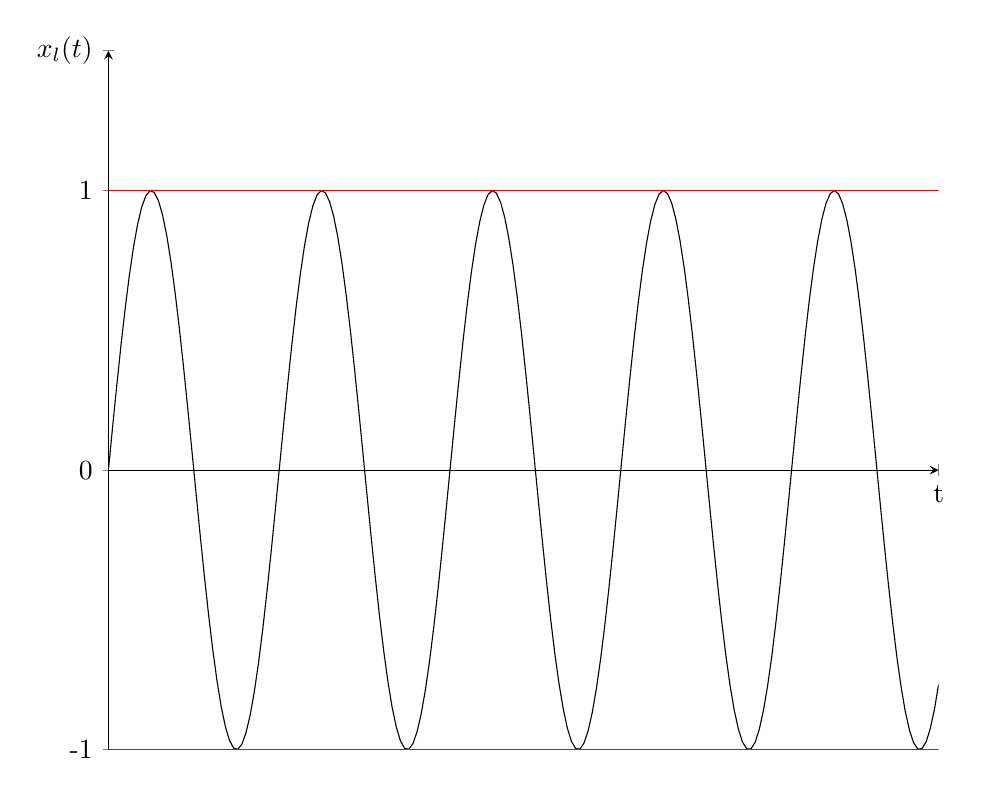
\begin{tikzpicture}
   \begin{axis}[
     axis lines=left,
     axis x line=middle,
     width=\textwidth,
     xtick={0,3.5},
     xticklabels={0,t},
     ytick={-1,0,1,1.5},
     ymax=1.5,
     ymin = -1,
     yticklabels={-1,0,1,$x_l(t)$},
     ]
    \addplot[color=black,domain=0:3.5,samples=200]{sin(500*x)};
    \addplot[color=red,domain=0:3.5]{1};
    \addplot[color=red,domain=0:3.5]{-1};
    \end{axis}
  \end{tikzpicture}
  \caption{$\alpha=0$}
 \end{subfigure}
\hfill
 \begin{subfigure}[b]{0.32\textwidth}
  \centering
  \begin{tikzpicture}
   \begin{axis}[
     axis lines=left,
     axis x line=middle,
     width=\textwidth,
     xtick={0,3.5},
     xticklabels={0,t},
     ytick={0,34},
     ymax=34,
     ymin = -34,
     yticklabels={0,$x_l(t)$},
     ]
    \addplot[color=black,domain=0:3.5,samples=200]{exp(x)*sin(500*x)};
    \addplot[color=red,domain=0:3.5]{exp(x)};
    \addplot[color=red,domain=0:3.5]{-exp(x)};
    \end{axis}
  \end{tikzpicture}
  \caption{$\alpha>0$}
 \end{subfigure}
\end{figure}

Nel caso di autovalori puramente immaginari si ha un andamento puramente
periodico e non pseudo-periodico.
Negli altri due casi la funzione esponenziale rappresenta la curva
\textit{inviluppo} della soluzione.

Lo spazio delle soluzioni $X^n$ è formato da una base di due vettori non
necessariamente ortogonali tra loro $u_a$ ed $u_b$, il vettore soluzione ruota
nel piano ottenuto dai vettori della base e la sua ampiezza può variare o meno
nel tempo a seconda del segno di $\alpha$.
Se $\alpha=0$ si ha genericamente un ellisse che collassa in una circonferenza
qualora i due assi fossero ortogonali e avessero la stessa ampiezza.

\begin{figure}[h]
\centering
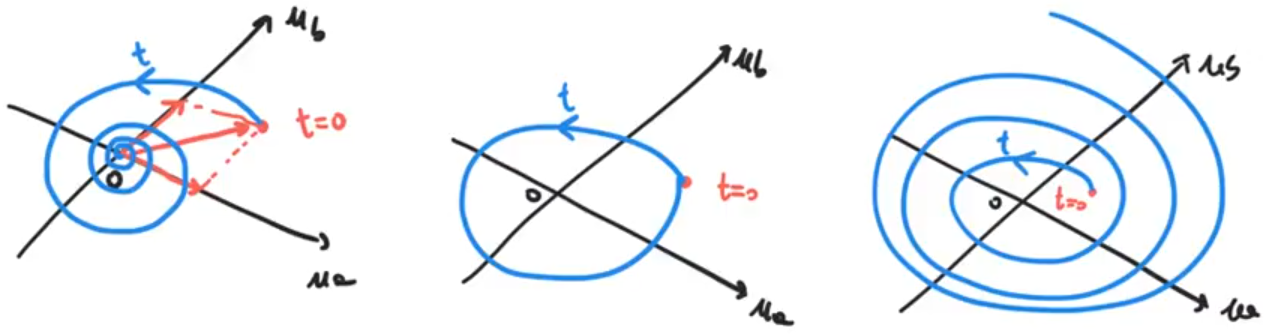
\includegraphics[width=0.8\linewidth]{andamento_soluzione_periodica}
\end{figure}

Due parametri che caratterizzano i modi pseudo-periodici sono
\begin{itemize}
\item \textbf{Pulsazione naturale} $\omega_n =
\sqrt{\alpha^2+\omega^2}$
\item \textbf{Coefficiente di smorzamento} $\zeta =
-\frac{\alpha}{\omega_n}$
\end{itemize}

\newpage
Dal punto di vista grafico
\begin{figure}[H]
\centering
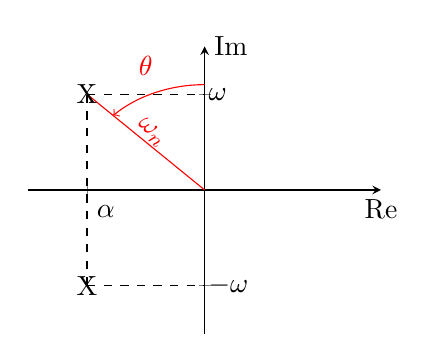
\begin{tikzpicture}
\begin{axis}[
    axis lines = middle,
    width = 0.5\linewidth,
    ymin = -1.5,
    ymax = 1.5,
    xmax = 1.5,
    xmin = -1.5,
    xticklabel style={anchor=north west},
    yticklabel style={anchor=west},
    xtick = {-1,0},
    xticklabels={$\alpha$, 0},
    ytick = {-1,0,1},
    yticklabels={$-\omega$,0,$\omega$},
    xlabel=Re,ylabel=Im,
    %axis line style={latex-latex},
    %axis line style={shorten >=-7.5pt, shorten <=-7.5pt},
    xlabel style={at={(ticklabel* cs:1)},anchor=north},
    ylabel style={at={(ticklabel* cs:1)},anchor=west},
]
\addplot[color=red,domain=-1:0]{-x};
\draw [dashed] (-1,-1) -- (-1,1);
\draw [dashed] (-1,-1) -- (0,-1);
\draw [dashed] (-1,1) -- (0,1);
\node[] at  (axis cs:-1,1){X};
\node[] at (axis cs:-1,-1){X};
\node[color=red,rotate=-44] at (axis cs:-0.45,0.6){$\omega_n$};
\draw [color=red,->] (0,1.1) arc (90:135:1.1);
\node[color=red] at (axis cs:-0.5,1.3){$\theta$};
\end{axis}
\end{tikzpicture}
\end{figure}
%figure
%\begin{figure}[H]
%\centering
%\includegraphics[width=\picwid]{posizione_autovalori}
%\end{figure}
Dalla figura si vede la relazione tra l'angolo $\theta$ e $\zeta$
$$\zeta = \sin\theta \in ]-1,1[$$

Se fosse pari a $\pm\frac{\pi}{2}$ i due autovalori
coinciderebbero in un unico punto, ossia si avrebbe un autovalore reale di
molteplicità due, negativo o positivo.

A parità di $\omega_n$, al diminuire di $\theta$, diminuisce lo smorzamento,
ossia le oscillazioni perdurano per più tempo.

\subsection{Stima dell'andamento qualitativo dei sistemi dinamici}
Analisi dell'evoluzione libera di un sistema del secondo ordine con una coppia
di autovalori reali, negativi e distinti.
$$
x_l(t) = e^{At} x_0 = Ue^{\Lambda t}U^{-1}x_0
$$
\begin{figure}[H]
\centering
\begin{tikzpicture}
\begin{axis}[
    axis lines = middle,
    width = 0.5\linewidth,
    height =0.3\linewidth,
    ymin = -0.5,
    ymax = 0.5,
    xmax = 1,
    xmin = -2.5,
    %axis equal,
    %xticklabel style={anchor=north west},
    yticklabel style={anchor=west},
    xtick = {-2,-1,0},
    xticklabels={$\lambda_2$,$\lambda_1$, 0},
    ytick = {0},
    yticklabels={0},
    xlabel=Re,ylabel=Im,
    %axis line style={latex-latex},
    %axis line style={shorten >=-7.5pt, shorten <=-7.5pt},
    xlabel style={at={(ticklabel* cs:1)},anchor=north},
    ylabel style={at={(ticklabel* cs:1)},anchor=west},
]
\end{axis}
\end{tikzpicture}
\end{figure}

Si può effettuare un cambio di variabili
$x=Uz$, $U^{-1}x_0=Z_l(0)$, dai due autovalori è possibile ricavare gli
autovettori per costruire la matrice modale $U = (u_1 \ u_2)$.

$$
x_l(t) = \left(e^{\lambda_1 t}u_1v_1^T+e^{\lambda_2 t}u_2v_2^T\right)x_0 =
z_1(0) e^{\lambda_1 t} u_1 + z_2(0)e^{\lambda_2 t}u_2
$$

\newpage
Si riporta l'andamento dello stato del sistema nel piano chiamato
\textit{ritratto di fase}

\begin{figure}[H]
\centering
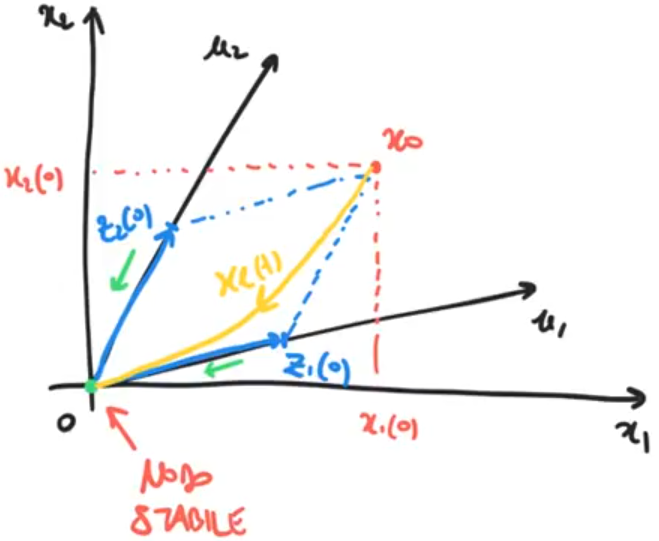
\includegraphics[width=\picwid]{traiettoria_stato_convergente}
\end{figure}

Entrambi i vettori si accorciano nell'origine, la traiettoria del punto $x_0$ è
contenuta nella regione di piano delimitata dai vettori $u_1$ ed $u_2$. Se gli
autovalori fossero uguali la traiettoria sarebbe rettilinea, ma $\lambda_1$ è
minore in modulo rispetto a $\lambda_2$ dunque la
sua costante di tempo sarà più grande, di conseguenza la traiettoria sarà curva
e vicina al vettore $u_1$.

Si dice che $\lambda_1$ è l'autovalore dominante perché perdura più a lungo nel
tempo, è sempre l'autovalore massimo.
L'origine è in questo caso un \textbf{nodo stabile} della traiettoria.

\subsubsection{Andamento con autovalori positivi}
Se gli autovalori sono positivi
\begin{figure}[H]
\centering
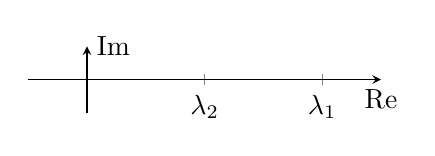
\begin{tikzpicture}
\begin{axis}[
    axis lines = middle,
    width = 0.5\linewidth,
    height =0.2\linewidth,
    ymin = -0.5,
    ymax = 0.5,
    xmax = 2.5,
    xmin = -0.5,
    %axis equal,
    %xticklabel style={anchor=north west},
    yticklabel style={anchor=west},
    xtick = {0,1,2},
    xticklabels={0,$\lambda_2$,$\lambda_1$},
    ytick = {0},
    yticklabels={0},
    xlabel=Re,ylabel=Im,
    %axis line style={latex-latex},
    %axis line style={shorten >=-7.5pt, shorten <=-7.5pt},
    xlabel style={at={(ticklabel* cs:1)},anchor=north},
    ylabel style={at={(ticklabel* cs:1)},anchor=west},
]
\end{axis}
\end{tikzpicture}
\end{figure}

Anche in questo caso l'autovalore dominante è $\lambda_1$, ossia la
componente ad esso associato diverge più rapidamente di quella
associata all'autovalore $\lambda_2$, la traiettoria tenderà ad una retta
parallela ad $u_1$
\begin{figure}[h]
\centering
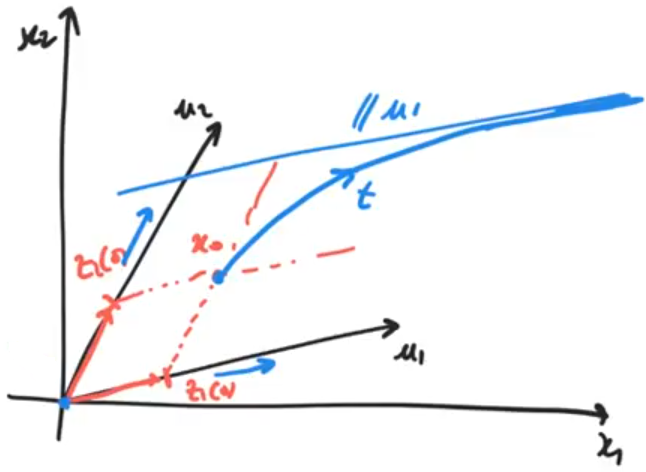
\includegraphics[width=\picwid]{traiettoria_stato_divergente}
\end{figure}

L'origine viene definito in questo caso un \textbf{nodo instabile} dato che le
componenti si allontanano da quel punto.

\newpage
\subsubsection{Autovalori con segno discorde}
Nel caso in cui gli autovalori fossero di segno opposto, si avrebbe ancora
$\lambda_1$ come autovalore dominante, mentre il secondo tenderebbe a zero
\begin{figure}[H]
\centering
\begin{tikzpicture}
\begin{axis}[
    axis lines = middle,
    width = 0.5\linewidth,
    height =0.3\linewidth,
    ymin = -0.5,
    ymax = 0.5,
    xmax = 1.5,
    xmin = -1.5,
    %axis equal,
    %xticklabel style={anchor=north west},
    yticklabel style={anchor=west},
    xtick = {-1,0,1},
    xticklabels={$\lambda_2$,0,$\lambda_1$},
    ytick = {0},
    yticklabels={0},
    xlabel=Re,ylabel=Im,
    %axis line style={latex-latex},
    %axis line style={shorten >=-7.5pt, shorten <=-7.5pt},
    xlabel style={at={(ticklabel* cs:1)},anchor=north},
    ylabel style={at={(ticklabel* cs:1)},anchor=west},
]
\end{axis}
\end{tikzpicture}
\end{figure}
La traiettoria tende a coincidere alla retta determinata da $u_1$.
\begin{figure}[H]
\centering
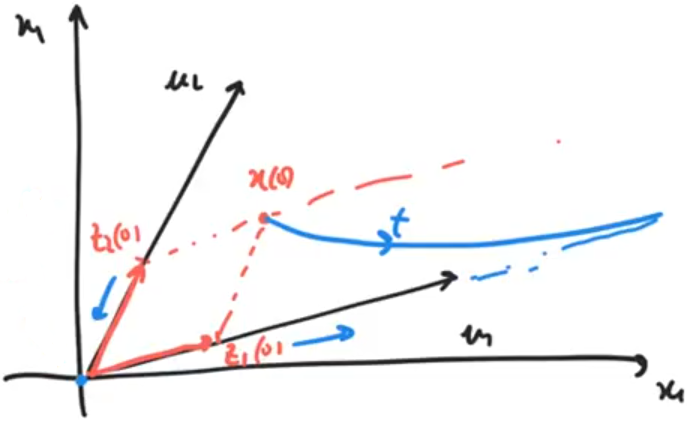
\includegraphics[width=\picwid]{traiettoria_stato_sella}
\end{figure}
L'origine verrà detto \textbf{punto di sella} a causa del diverso comportamento
rispetto alle due componenti.
